\section{Folosirea în contextul demonstraţiilor de concept a DVM versiunea 1}

Prima versiune a mediatorului cu valori implicite a fost o unealtă foarte importantă în contextul celei de-a doua demonstraţii de concept a proiectului rețelelor de transport de date fără fir din cadrul \gls{onf}. Acesta a ajutat la accelerarea implementării aplicațiilor \gls{sdn} care au fost dezvoltate pentru cazurile de utilizare propuse în \cite{onf2016_poc2}.

\gls{dvm} a oferit interfaţa de Sud \gls{netconf} care expune modelele informaționale dezvoltate de \gls{onf}, în același mod în care ar expune-o un mediator real ce se conectează la echipamente de transport de date fără fir. În acest mod, dezvoltatorii aplicațiilor \gls{sdn} au putut utiliza acest simulator pentru implementarea și testarea acestora, fără a avea nevoie să deţină dispozitive de rețea, care au un preţ foarte ridicat.

Această primă versiune de simulator a accelerat activitățile de pregătire a celei de-a doua demonstraţii de concept, permiţând lucrul în paralel la aplicațiile \gls{sdn} și la dezvoltarea mediatoarelor. Interfaţa \gls{netconf} comună a putut fi testată înainte ca producătorii de echipamente să își implementeze mediatoarele, oferind astfel mai mult timp dezvoltatorilor aplicațiilor \gls{sdn} pentru depanarea programelor. De exemplu, generarea unei notificări \gls{netconf} se poate face mult mai facil cu ajutorul simulatorului. Pentru un mediator real, trebuie ca dispozitivul să fie făcut să genereze o notificare către mediator, prin interfaţa proprietară echipamentului respectiv, apoi mediatorul să traducă acel mesaj într-o notificare \gls{netconf}.

Figura \ref{fig:dvmv01_poc_usage} reprezintă elementele de bază ale demonstraţiei de concept, așa cum sunt prezentate în lucrarea apărută după desfăşurarea acestuia \cite{onf2016_poc2}, în care se poate vedea \gls{dvm}.

\begin{figure}[h]
	\centering
	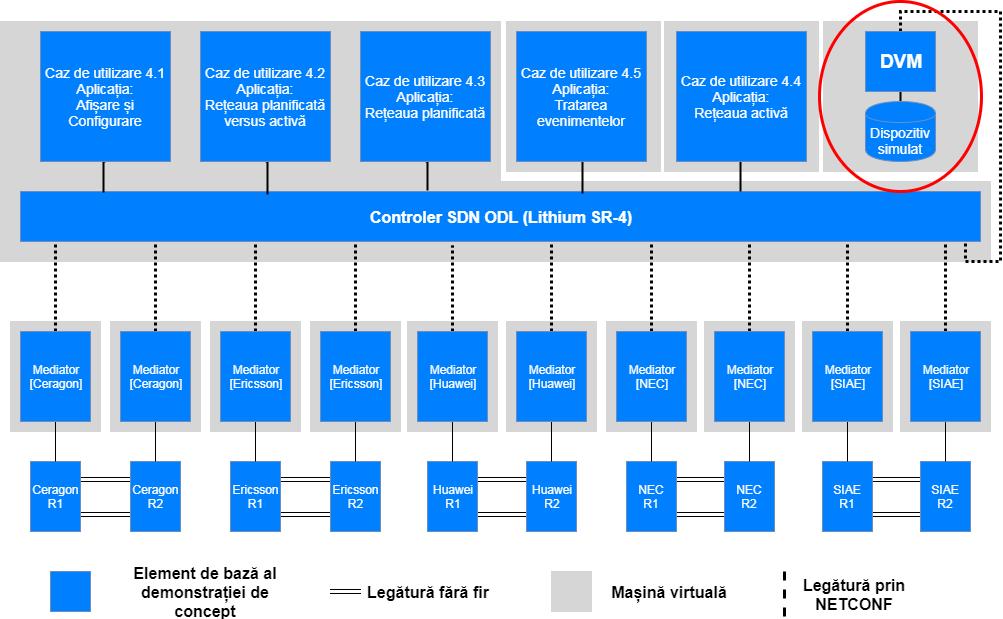
\includegraphics[width=1\textwidth]{dvmv01_poc_usage}
	\caption{Configurarea rețelei de test SDN utilizând mașini virtuale \cite{onf2016_poc2}.}
	\label{fig:dvmv01_poc_usage}
\end{figure}

Înregistrarea la controlerul \gls{sdn} a primei versiuni a simulatoarelor \gls{dvm}, se face la fel ca pentru un mediator real. Astfel, echipamentul de control oferă o \textit{interfață de programare a aplicaţiei} - \gls{api} - prin care o aplicație \gls{sdn} poate înregistra un astfel de mediator în controlerul \gls{sdn}. Înregistrarea nu este una automată, utilizatorul fiind nevoit să facă această înregistrare manual. În cea de-a doua demonstraţie de concept, acest lucru a fost făcut prin interfaţa grafică a echipamentului de control folosit (\gls{odl}). După înregistrare, controlerul stabileşte conexiunea \gls{netconf} cu mediatorul.

Codul asociat primei versiuni a \gls{dvm} este oferit cu sursă deschisă și se poate găsi în repertoriul asociat \gls{onf} de pe platforma GitHub, denumit CENTENNIAL \cite{dvmv01github}.